\section{Wstęp}
Za protoplastę tych (głębokich) sieci można uznać zdefiniowany na początku lat `90 wielowarstwowy neocognitron prof. Kunihiko Fukushimy. Prawdziwy rozwój tych sieci zawdzięczamy jednak profesorowi Yann A. LeCun, który zdefiniował podstawową strukturę i algorytm uczący specjalizowanej sieci konwolucyjnej CNN. Aktualnie sieci CNN stanowią podstawową strukturę stosowaną na szeroką skalę w przetwarzaniu sygnałów i obrazów. W międzyczasie powstało wiele odmian sieci będącej modyfikacją struktury podstawowej (R-CNN, AlexNET, GoogLeNet, ResNet, U-Net, YOLO)\cite{Osowski2023}.\\
Sieci CNN powstały jako narzędzie analizy i rozpoznawania obrazów wzorowanym na sposobie działania naszych zmysłów. Wyeliminowały kłopotliwy proces manualnego opisu cech charakterystycznych obrazów. W tym rozwiązaniu sieć sama odpowiada za generację cech charakterystycznych dla klas \cite{Osowski2023}. Przetwarzania obrazu przez zestaw filtrów i warstw generuje obrazy o coraz mniejszych  wymiarach, lecz o zwiększającej się liczebności kanałów reprezentujących cechy charakterystyczne dla przetwarzanego zbioru. Próbka danych w kolejnych etapach jest reprezentowana przez tensory (struktury trójwymiarowe, których szerokość i wysokość odpowiada wymiarom obrazu, a głębokość jest równa liczbie kanałów w obrazie). Wyjście z ostatniej warstwy sieci w procesie wypłaszczania jest przetwarzane na postać wektorową (jednowymiarowa tablica liczb), a następnie przekazywane na wejście układu klasyfikującego - sieci MLP z wyjściem Softmax \cite{YannCnn} \cite{Qi2016DerivationOB}.


%\href{2016.10 - Derivation of Backpropagation in Convolutional Neural Network (CNN).pdf}

%\href{https://zzutk.github.io/docs/reports/2016.10%20-%20Derivation%20of%20Backpropagation%20in%20Convolutional%20Neural%20Network%20(CNN).pdf}

%\href{https://www.bibsonomy.org/bibtex/28d520c74cb5aeee1bcae26642b7d973d/tobias.koopmann}



%Convolution !
%\href{https://arxiv.org/pdf/1603.07285}


%Back convolution
%\href{https://hal.science/hal-04409232/document}

~
\newline
\begin{figure}[ht]
    	\centering 
            \includegraphics[width=0.90\linewidth]{rysunki/Lecun98-7.jpg} 
            \caption{Architektura LaNet-5 \cite{YannCnn}}
\end{figure} 
\newpage 
\begin{figure}[ht]
    	\centering 
            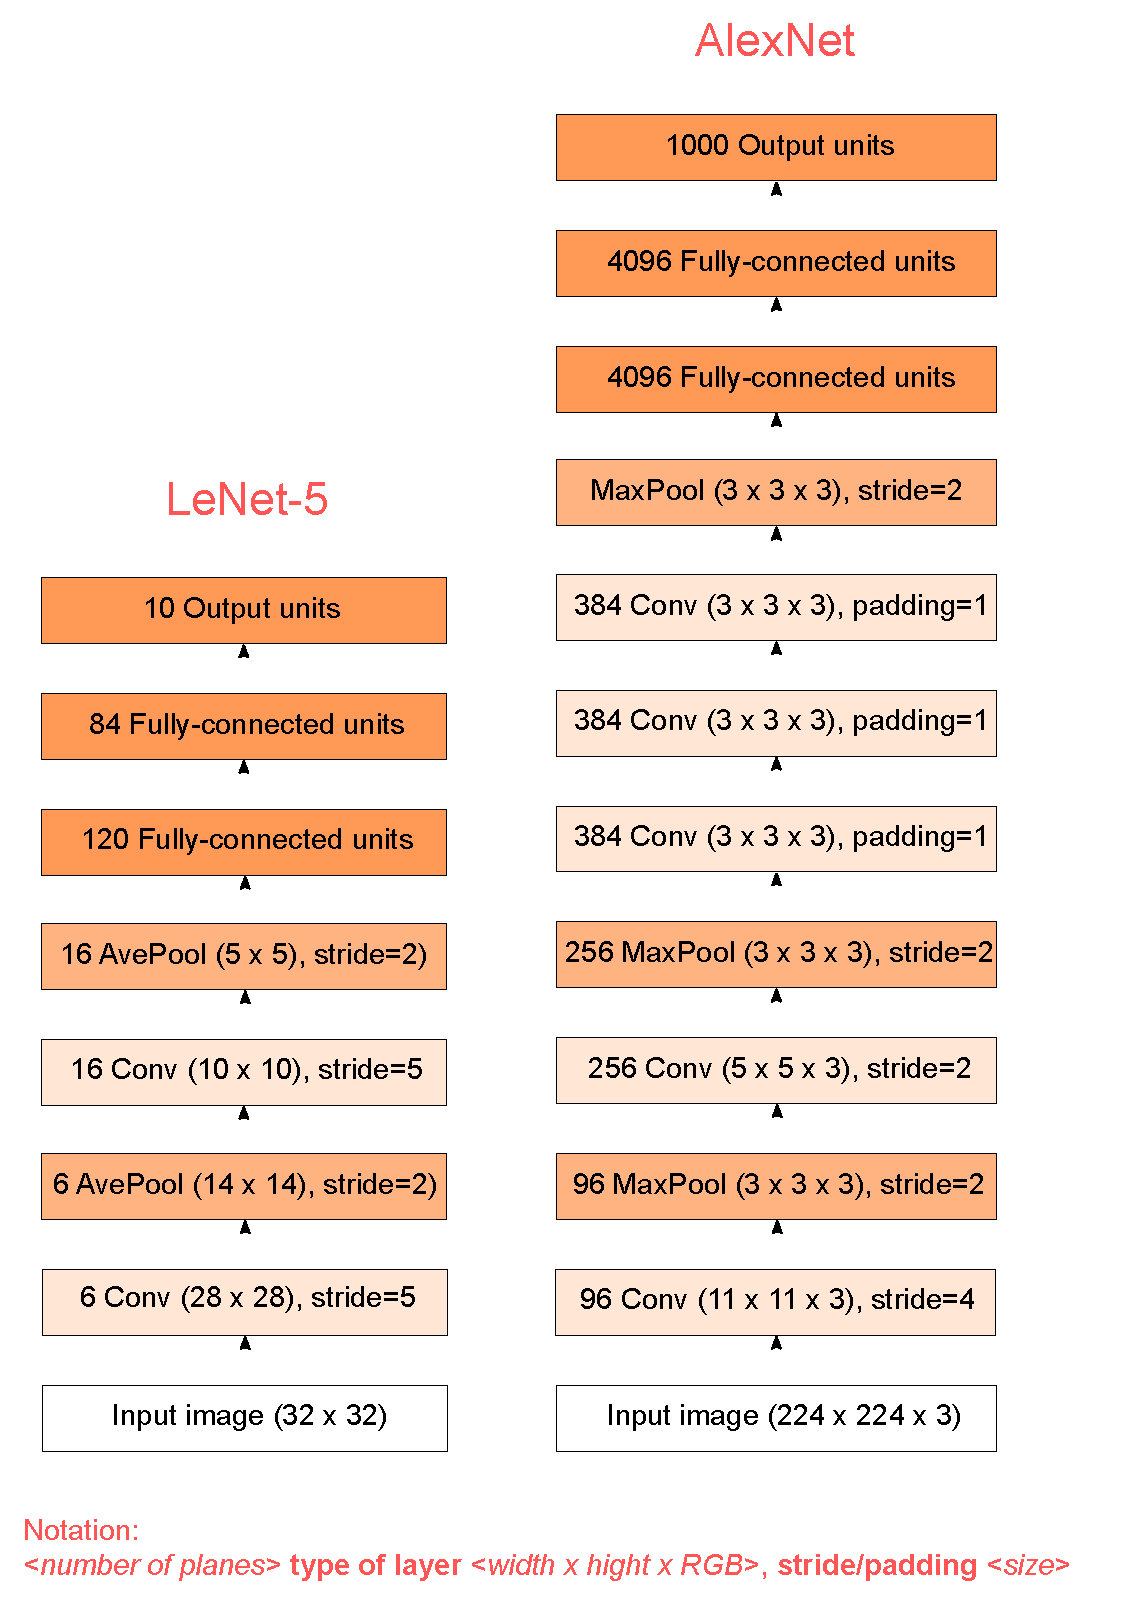
\includegraphics[width=0.70\linewidth]{rysunki/alexnet.jpg} 
            \label{fig:lanet}
            \caption{Porównanie struktury LaNet i AlexNet \cite{strAlexnet} }
\end{figure} 
\newpage 

 
\section{Operacja splotu }
Jeśli wartości pikseli obrazu wejściowego \(X\)
oznaczymy \(X_{(i,j)}\), a wartości filtra \(F\) oznaczymy jako \(F_{(m,n)}\) obraz wejściowy \(Y\), \(Y_{(o,p)}\), wówczas każdy piksel obrazu wyjściowego obliczymy:

\begin{equation}
      Y_{(O,P)} = \sum _{(n=1)} ^{(N)} 
                  \sum _{(m=1)} ^{(M)} 
                  F_{(m,n)}*X_{(m+O,n+P)}
\end{equation} 

\begin{figure}[ht]
    	\centering 
            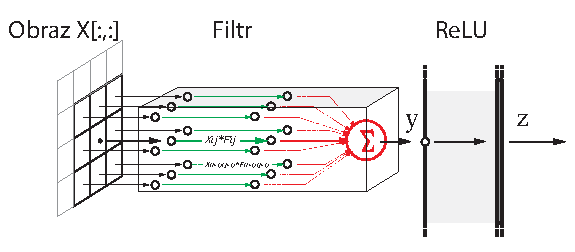
\includegraphics[width=0.70\linewidth]{rysunki/rys2_1.jpg} 
            \caption{Obliczanie wartości pojedynczego piksela w procesie splotu analogicznie jak w MLP, sprowadza się do obliczenia sumy ważonej piksela centralnego filtra z pikselem obrazu oraz najbliższych sąsiadów centralnego piksela - tych które znajdują się naprzeciw pikseli filtra. }
\end{figure} 
\subsection{Padding}

\begin{figure}[ht]
    	\centering 
            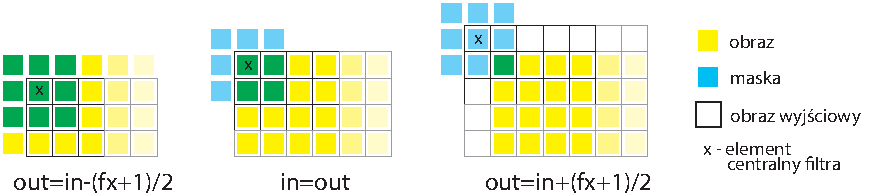
\includegraphics[width=0.99\linewidth]{rysunki/rys2_2.jpg} 
            \caption{Wpływ punktu startowego maski na wymiar obrazu wynikowego operacji splotu }
\end{figure} 
Padding oznacza wysunięcie maski poza obszar obrazu. \newline Jeśli w procesie konwolucji centralny piksel maski:
\begin{itemize}
    \item 
    znajduje się przed granicą obrazu, wówczas obraz wynikowy będzie mniejszy (p>0).
    
    \item 
    znajduje się nad pierwszym pikselem obrazu, wówczas wielkość obrazu wyjściowego jest taka jak obrazu wejściowego (p=0).

    \item 
    znajduje się poza pikselem obrazu, wówczas wielkość obrazu wyjściowego będzie większa (p<0).
    
\end{itemize}

W założeniu procesu uczenia, każdy przesyłany sygnał wejściowy i wyjściowy jest sprzężony z powrotnym sygnałem określającym wielkość błędu tego sygnału. Zatem jeśli w operacji splotu padding jest dodatni, wówczas przy obliczeniu błędu wyjściowego zastosowany będzie padding ujemny.


\subsection{Stride}
%Stride oznacza skok o ile pikseli przesuwa się maska w jednym kroku.
\begin{figure}[ht]
    	\centering 
            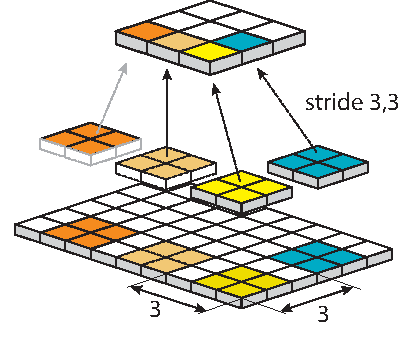
\includegraphics[width=0.4\linewidth]{rysunki/conv4a.jpg} 
            \caption{Stride, krok przesunięcia maski}
\end{figure} 

Wymiar wyjściowy obrazu  \(dimOut = ( dimIn + 1 - dimF + 2*padding ) / stride \) 
\begin{figure}[ht]
    	\centering 
            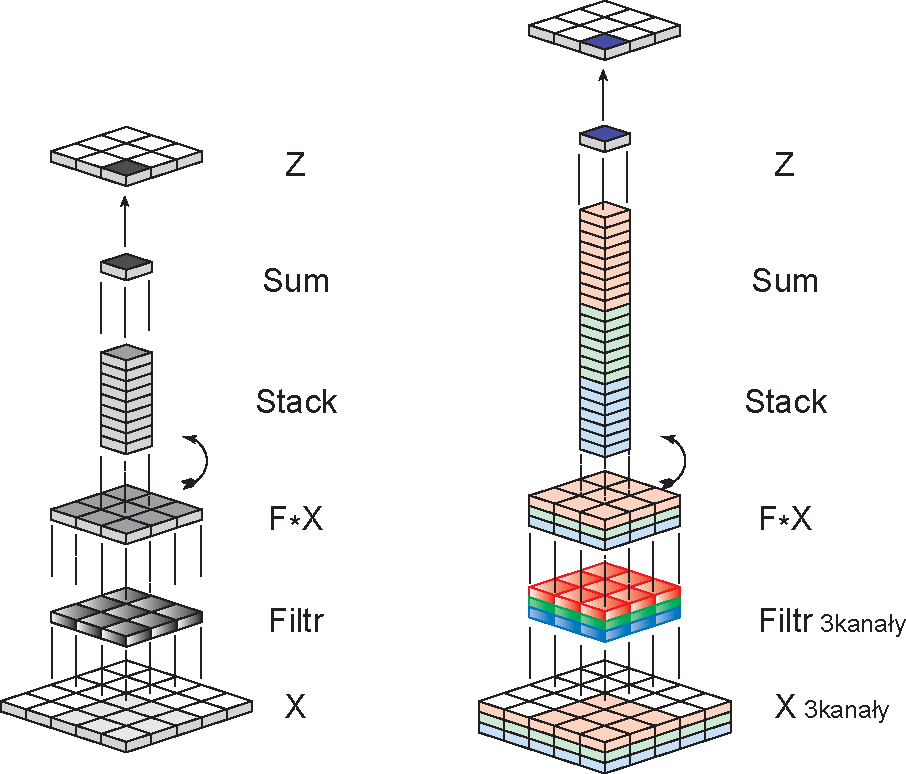
\includegraphics[width=0.76\linewidth]{rysunki/conv2b.jpg} 
            \caption{Konwolucja jedno i wielokanałowa}
\end{figure} 




\newpage
\section{ReLU i warstwy redukujące wymiar }

\begin{figure}[ht]
    	\centering 
            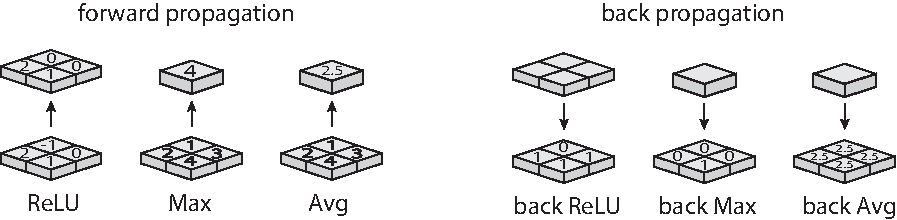
\includegraphics[width=0.95\linewidth]{rysunki/conv3.jpg} 
            \caption{Wynik działania warstw ReLU, Avg, Max przy przepływie wprost i wstecz.  }
\end{figure} 
Po operacji splotu można zastosować warstwę ReLU. Funkcja aktywacji ReLU = max\{x, 0\}. Zerowane są wartości ujemne, funkcja nie ma ciągłej pochodnej, przy obliczeniach przyjmowano że pochodna wynosi 1 gdy wartość wyjścia z była większa od 0, lub 0 jeśli wartość z była mniejsza od zera.\newline
Można także zastosować warstwy redukującą rozmiar. Warstwa AVG - na wyjściu zwraca średnią wartości sąsiednich pól; pochodna przy przepływie wstecz dla każdego pola wynosi \(1/n^2\) gdzie n jest wielkością filtra. Warstwa MAX - na wyjściu zwraca wartość maksymalną z pól objętych zasięgiem filtra. Pochodna przy propagacji wstecz wynosi 1 dla wartości maksymalnej i 0 dla pozostałych.  

\section{Przetwarzanie w przód }
Obraz wejściowy w skali szarości, lub obraz kolorowy rozbity na 3 kanały RGB zostaje przetworzony w operacji splotu przez grupy warstw filtrów i warstwy redukujące. Warstwa konwolucyjna może zmniejszyć, a warstwa redukująca zawsze zmniejsza rozmiar obrazu, w efekcie otrzymujemy coraz mniejsze obrazy wyjściowe. \newline
Wyjściem każdego filtra jest jeden kanał obrazu. W miarę zmniejszania obrazów stosowana jest większa liczbę filtrów, co zwiększa liczbę kanałów. Przedostatnia warstwa spłaszcza wszystkie kanały obrazu do postaci pojedynczego jednowymiarowego wektora, warstwa ostatnia Full Connected z~wyjściem Softmax dokonuje klasyfikacji obrazu.
 

\section{Przetwarzanie wstecz - modyfikacja filtra w warstwie splotowej }
Wektor wielkości błędu zostaje przekazany z warstw MLP przez warstwy redukujące do warstw splotowych, w których następuje modyfikacja Filtra zgodnie z formułą.

\begin{equation}
    \frac{\partial L}{\partial F} = Conv( Input.X , Loss.Gradient \frac{\partial L}{\partial O} ) ; 
    F=F-\mu * \frac{\partial L}{\partial F}
\end{equation}
\begin{equation}
    \frac{\partial L}{\partial Bias} = Sum( Loss.Gradient \frac{\partial L}{\partial O} ) ; 
    Bias=Bias-\mu * \frac{\partial L}{\partial Bias}
\end{equation}

\section{Propagacja błędu przez warstwę splotową }
Do warstwy poprzedniej zostanie przekazany wektor błędu o wartości wyliczonej wg. wzoru:

\begin{equation}
    \frac{\partial L}{\partial X} = FullConv( 180Rotated.filter.F, Loss.Gradient \frac{\partial L}{\partial O } )  
\end{equation}